This thesis detailed the HWW VBF fiducial cross-section analysis as it currently stands, but there are further developments still underway. This analysis plans to measure differential cross-sections and the full unfolding procedure is almost complete. In addition, Chapter 6 discussed some theoretical uncertainties (VBF and ggF Higgs as well as top, WW, and $Z\rightarrow \tau\tau$) that are currently estimated through global floating values. In our final analysis, the uncertainties shape effects will be taken into account as well as their normalization variations.

\section{Outlook: differential cross-section measurements}
The differential cross-section measurement requires a more rigorous unfolding procedure than the total fiducial and inclusive cross-sections. Monte Carlo simulations processed in a pseudo-detector with all its expected inefficencies and limits (detector-level) are compared to Monte Carlo simulations processed solely at the particle-level. This analysis will employ the iterative Bayesian unfolding method \cite{bayesian} whose goal is to determine the probability that each bin in a detector-level distribution corresponds to a bin in a particle-level distribution. 
%Using Bayes' theorem, this probability can be attained with knowledge of the true spectrum $T$ and the measured or reco-level spectrum $R$. We begin with Bayes' theorem: 
%\begin{equation}
%P(T_i|R)=\frac{P(R,T_i)P(T_i)}{\sum_{t} P(R,T_t)P(T_t)},
%\end{equation}
%where the denominator is a normalization factor, $P(R,T_i)$ represents the likelihood and $P(T_i)$ the prior. The prior here is indeterminant and so we begin with the assumption that $P(T_i)$ is constant. Hence the most probable spectrum for $T$ maximizes the likelihood. If we observe $n$ reco-level events, we can assign the probability of their true distributions through
%\begin{equation}
%\hat{n}(T_i)=n(R)\prod P(T_i|R).
%\end{equation}
%We then use resultant possibilities in the Bayes formula to evaluate $P(T_i|R_j)$. These values constitute the smearing matrix $M$. This matrix can be used to estimate the truth-level events in each bin of a distribution with
%\begin{equation}
%\hat{n}(T_i)=\frac{1}{\epsilon_i}\sum_{j=1}^{n_R} n(R_j)\prod P(T_i|R_j),
%\end{equation}
%where $\epsilon$ is the inefficiency, or ratio of events that pass both truth and reco-level selection by those that pass only truth. Finally the truth can be determined by the reconstructed bin-by-bin yields through
%\begin{equation}
%n(T_i)=\sum_j M_{ij} \prod n(R_j).
%\end{equation}
%The migration matrix directly maps reco-level distributions to truth-level. In order to calculate this matrix iteratively we first allow $P(T_i)$ to be a constant distribution, say $1/n_T$, which gives an expected number of truth events $n_0(C_i)=P_0(C_i)\prod n_R$. Next, we calculate $\hat{n}(C)$ using the efficiency equation, and finally we use a $\chi^2$ to compare $\hat{n}(C)$ and $n_0(C)$. In the next iteration, $n_0$ is replaced by $\hat{n}$ and $P_0$ by $\hat{P}$, $\hat{P(C_i)}=\hat{n}(C_i)/\hat{N_{true}}$, and the procedure continues until the $\chi^2$ falls below a set threshold. 

%While the final unfolding results fall beyond the scope of thesis, results for four kinematic variables are shown in Figure~\ref{fig:unfoldingmatrices}. We use reconstruction-level Monte Carlo events and their truth counterparts to calculate migration matrices for each differential observable through the iterative Bayesian unfolding process. 

%\begin{figure}[!h]
%\centering
%  \subfloat[$p^T_H$]{
%      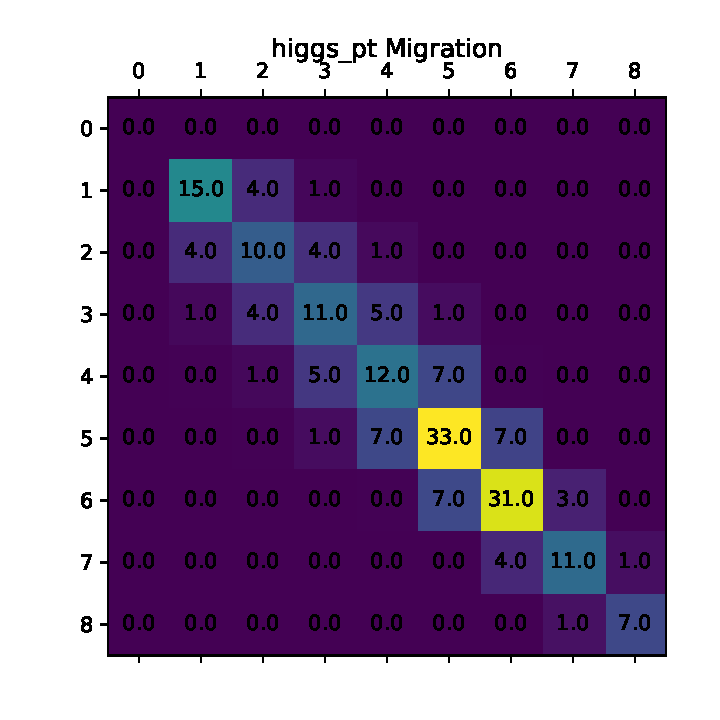
\includegraphics[width=.4\textwidth]{Pictures/unfolding/response_matrices/higgs_pt_migrations.pdf}
%  }\hfill
%  \subfloat[$m_T^{\ell\ell}$]{
%      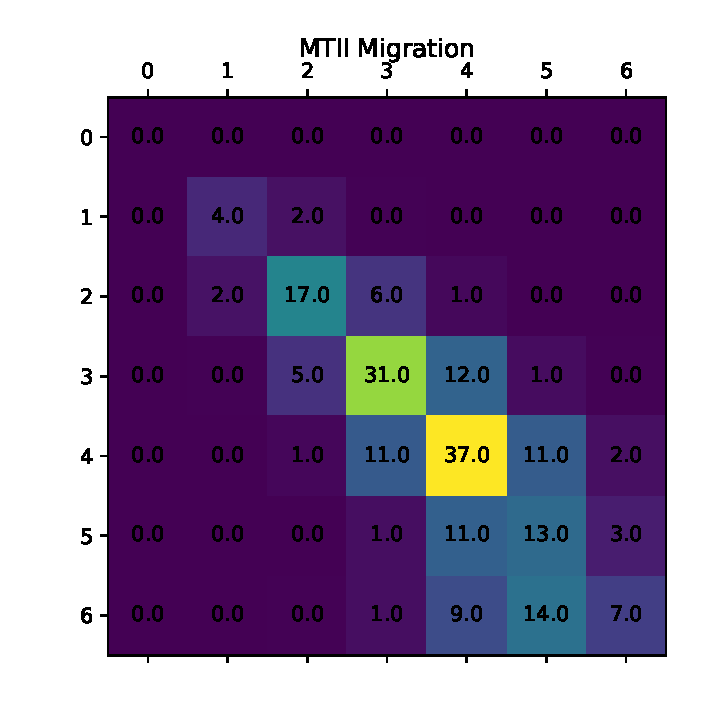
\includegraphics[width=.4\textwidth]{Pictures/unfolding/response_matrices/MTll_migrations.pdf}
%  }\hfill
%  \subfloat[$\Delta Y_{\ell\ell}$]{
%      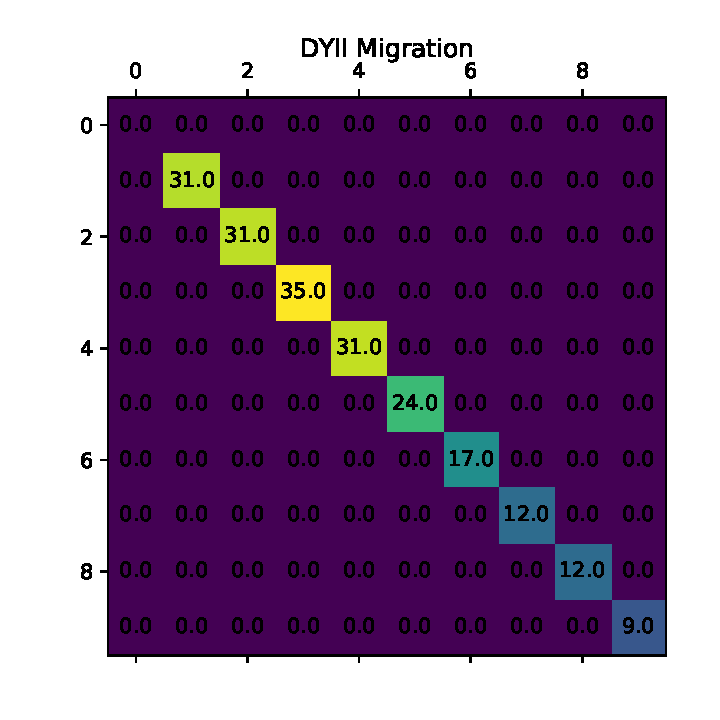
\includegraphics[width=.4\textwidth]{Pictures/unfolding/response_matrices/DYll_migrations.pdf}
%  }\hfill
%  \subfloat[$m_{jj}$]{
%      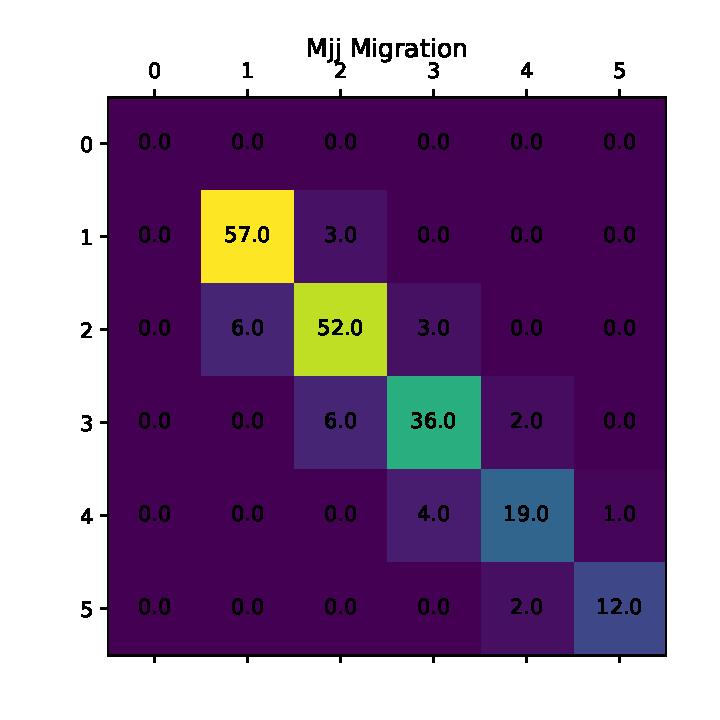
\includegraphics[width=.4\textwidth]{Pictures/unfolding/response_matrices/Mjj_migrations.pdf}
%  }%hfill
%\caption{\label{fig:unfoldingmatrices}Unfolding matrices shown for $p^T_H$, $m_T^{\ell\ell}$, $\Delta Y_{\ell\ell}$ and $m_{jj}$ distributions. Each bin value corresponds to normalized Bayesian probabilities and the x-axis represents reconstruction-level distributions while the y-axis shows truth distributions~\cite{ourSupportNote}.\textcolor{red}{Will replace with brighter images}}
%\end{figure}  

Developments in unfolding are underway currently and include estimating error added by the procedure, testing for potential biases toward the particle-level distribution, and understanding unfolding detector-level uncertainties as well as nominal distributions. 

Signal and background yields will be used within the unfolding mechanism to extract final differential distributions. The variables used in the differential analysis will also be finalized in coming months, but will certainly include $m_{jj}$ and $\Delta Y_{jj}$. These variables probe the kinematics of the final state particles measured through this channel and add sensitivity to the total fiducial and inclusive cross-sections. The invariant mass of the two jets that accompany the $W$ bosons ($m_{jj}$) and the angular separation between them ($\Delta y_{jj}$) are particularly sensitive to the electroweak symmetry breaking mechanism. Deviations between data and theoretical predictions in the distribution of these variables may be signs of new physics that alter the HWW coupling, like new resonances at high energy scales not accessible by direct searches.                

%\begin{table}[h!]
%\begin{center}
%\begin{tabular}{ |c||c|  }
% \hline
% Observable & Bin Edges\\
% \hline
% $MT^{l,l,MET}$ &15,40,65,80,95,110,115,120,180\\
% $Mll$&  0,20,25,30,35,40,45, 50, 60, 70,200\\
% $Mjj$ &200,450,700,950,1200,1500,2200,3000,5000\\
% $Cos(\theta^{*})$ &0,0.125,0.25,0.375,0.5,0.625,1.0\\
% $DYll$&   0,0.15,0.3,0.45,0.6,0.75,0.9,1.05,1.2,1.5,4\\
% $DYjj$& 0,2.5,3.25,3.62,4,4.35,4.75,5,5.5,6.25,7,8.5\\
% $P_{t}$ Total& 150,200,250,350,500,600,900\\
% $DPhill$& 0,0.1,0.2,0.3,0.4,0.6,0.8,1.0,1.3,1.7,2.1,2.6,3.2\\
% $P_{t} ll$&0,20,40,50,60,70,80,90,100,120,160,500\\
% Higgs $P_{t}$&0,45,80,120,160,200,260,350,1000\\
% Leading Lepton $P_{t}$&20,25,35,42,50,65,80,90,2000\\
% Subleading Lepton $P_{t}$&20,25,35,42,50,65,80,90,2000\\
% Leading Jet $P_{t}$&30,60,90,120,190,260,350,500\\
% Subleading Jet $P_{t}$& 30,60,90,120,190,260,350\\
% \hline
%\end{tabular}
%\end{center}
%\caption{Planned observables and bin edges for differential cross-section measurements}
%\label{tab:observablebins}
%\end{table} 

%This analysis uses the full Run 2 dataset for VBF HWW cross-sections and new statistical methods. These have led to expected results which demonstrate large increases in sensitivity with respect to the most recent measurements. The VBF differential cross-sections measured for $H\rightarrow WW^*\rightarrow\ell\nu\ell\nu$ will be the first analyzed with the ATLAS experiment. 

%This analysis has an additional motivation as well. It is the first step in a larger measurement of both the VBF HWW differential cross-section and the Standard Model VBF $W+jj$ production cross-section. In the $W+$ jets production in the $\ell+$jets final state, the invariant mass of the two jets that accompany the $W$ bosons and the rapidity separation between them are particularly sensitive to the electroweak symmetry breaking mechanism just as in the VBF HWW cross-section. The final-state jets also have similar kinematics. Therefore the ratio of cross sections measurement allows for the cancellations of correlated systematic uncertainties. As both process are characterized by large ($10\%-20\%$) jet-related uncertainties, a reduction via the ratio cancellation would greatly improve the sensitivity to the VBF Higgs process and to the search for new phenomena in the context of EFT. This ratio measurement falls beyond the scope of this thesis but represents a complementary motivation to the measurements shown here. 

%In the context of vector boson scattering and with minimal assumptions on new physics, new phenomena are expected at a scale ($\Lambda$) higher than the one accessible by the experiment. These simultaneously effect $HWW$ and $WWV$ vertices. In particular, dimension-6 operators affect VBF Higgs mechanisms and VBF $W$ production, while the interplay of VBF and VBS mechanisms allows for the probe of dimension-6 and dimension-8 operators. The sensitivity to new physics is enhanced with precision-level measurements of fiducial and differential ratios of cross sections. Specifically, new phenomena that simultaneously affect both vertices are suppressed in the ratio of VBF Higgs to VBF $Wjj$ production, thus enhancing the sensitivity the phenomena affecting the $WWV$ vertex, for example. Similarly enhanced sensitivity can be achieved for anomalous quadruple-gauge couplings via the study of VBF Higgs and VBS $W$ productions. This ratio measurement between the two cross-sections is planned after publication of the VBF HWW differential cross-sections.
\section{Conclusion}

The Higgs boson was discovered in 2012 by the ATLAS and CMS collaborations. This heralded in a new era in high-energy physics. We know the Higgs boson exists, but have not yet precisely measured many of its properties. If these properties deviate from theory even slightly, there could be signs of new physics. Thus, the goals of the experiments have shifted---from discovery of a predicted Standard Model particle to the precise measurement of its various characteristics. 

This thesis focuses on the measurement of one such Higgs boson property, its fiducial cross-section with the VBF production mode in the $WW^*\rightarrow\ell\nu\ell\nu$ channel. This production mode is rare, only about $7\%$ of Higgs production, and previous measurements of VBF Higgs cross-sections in the $WW^*$ channel have associated uncertainties over $50\%$, far above those associated with ggF Higgs production~\cite{HWW2016}. The VBF Higgs production mode has a clear signal with its two associated jets, but even in a targeted fiducial region, contaminating backgrounds from $t\bar{t}$, ggF Higgs, and $Z\rightarrow\tau\tau$ are large. The $WW^*\rightarrow \ell\nu\ell\nu$ channel is chosen for its high branching ratio and clean lepton signature. We measure opposite flavor leptons (muons and electrons) to lower the contamination of Drell-Yan events. This analysis also uses sophisticated statistical approaches to control and mitigate the effects from each background. We measure expected mis-identified lepton backgrounds with a data-driven method, and use several optimized BDT discriminants to isolate ggF, top, and diboson backgrounds. Our measurement also benefits from 139 fb$^{-1}$ of recorded luminosity, a factor four greater than that used in the previous analysis. Although our sample size has increased substantially, statistical uncertainties still outweigh the impact from any other systematic. Finally, we carefully choose a fiducial region based on signal region cuts that amplify VBF events above their expected backgrounds and use particle-level MC simulations to translate our cross-section measured in the reconstructed ATLAS detecter to one which can be compared to theoretical estimations and other experimental measurements. Table~\ref{tab:comparison} compares results from the 36.1 fb$^{-1}$ measurement in Ref.~\cite{HWW2016} to the 139 fb$^{-1}$ measurement detailed in this thesis. The fiducial cross-sections cannot be compared directly as the fiducial phase space differs for each analysis. However, this measurement has substantially higher significance, with high enough certainty to be considered a discovery. The new experimental techniques used in this analysis, including the use of boosted decisions trees and optimized signal and control region selections, lead to the sizable decrease in systematic uncertainty in our result. 

\begin{table}[!h]
  \begin{center}
    \begin{tabular}{|l|c|c|}
       \hline
        Luminosity & 36.1 fb$^{-1}$    & 139 fb $^{-1}$ \\
      \hline
	Fiducial cross-section & --- & 2.78 fb \\ 
	Total uncertainty (\%) & +58/-56 & +20/-20 \\
	Statistical uncertainty (\%) & +48/-44 & +17/-16 \\
        Theoretical uncertainty (\%) & $\pm$26 & $\pm$10 \\
        Experimental uncertainty (\%) & $\pm$20 & +4/-5 \\
        Observed significance & 1.8$\sigma$& 6.6$\sigma$ \\
	\hline 
    \end{tabular}
    \caption{Comparison of measurements of VBF $H\rightarrow WW^*$ fiducial cross-sections using 36.1 fb$^{-1}$ and 139 fb$^{-1}$ measured in this thesis \cite{HWW2016}.}
    \label{tab:comparison}
  \end{center}
\end{table}

The fiducial cross-section measurement, 
\begin{equation}
\sigma_{\text{fid,obs}} = 2.78^{+0.56}_{-0.53} \text{ fb},
\end{equation}
is compatible with its Standard Model expectation of $2.67\pm0.004$~fb. The observed significance of $6.6\sigma$ demonstrates extremely high confidence that our measured Higgs signature is not a statistical fluctuation. The inclusive cross-section measurement,
\begin{equation}
89.2^{+18.3}_{-17.3} \text{ fb},
\end{equation}
also agrees with its Standard Model expectation, 85.8$\pm 3.1$~fb. 

Our increased precision measurements find no sizable deviation from the Standard Model, but the search continues. These measurements are the first part of a larger effort to measure differential cross-section distributions. These differential measurements will further increase sensitivity to new physics by detecting potential effects in distributions that are not visible in total cross-section values. The measurement of fiducial and inclusive VBF cross-sections is also certain to become more precise as the LHC records data in Run 3 and beyond. 
